\documentclass[dvipdfmx]{jarticle}
\pagestyle{empty}
\usepackage{tikz}
\newcommand{\greentext}[1]{{\color[rgb]{0,0.5,0}{#1}}}
\newcommand{\redtext}[1]{{\color[rgb]{0.8,0,0}{#1}}}
\newcommand{\bluetext}[1]{{\color[rgb]{0,0,0.8}{#1}}}

\newcommand{\tuple}[1]{\langle{#1}\rangle}

\newcommand{\First}{\mathsf{First}_1}
\newcommand{\Follow}{\mathsf{Follow}_1}

%%pdt simulation

\newcommand{\pdtline}[6]{%
    \uncover<#6->{
        \node at (${#5}*(0,-.3)+(0,.3)$) {$\vdash$};%
        \node at (${#5}*(0,-.3)+(1.5,.3)$) {\parbox{12em}{(#1,}};%
        \node at (${#5}*(0,-.3)+(4.5,.3)$) {\parbox{10em}{#2,}};%
        \node at (${#5}*(0,-.3)+(5.7,.3)$) {\parbox{10em}{#3)}};%
        \node at (${#5}*(0,-.3)+(8,.3)$) {\parbox{20em}{#4}};%
    }
}

\newcommand{\initpdtline}[6]{%
    \uncover<#6->{
        \node at (${#5}*(0,-.3)+(1.5,.3)$) {\parbox{12em}{(#1,}};%
        \node at (${#5}*(0,-.3)+(4.5,.3)$) {\parbox{10em}{#2,}};%
        \node at (${#5}*(0,-.3)+(5.7,.3)$) {\parbox{10em}{#3)}};%
        \node at (${#5}*(0,-.3)+(8,.3)$) {\parbox{20em}{#4}};%
    }
}

\newtheorem{Def}{定義}
\newtheorem{Lem}{補題}
\newtheorem{Thm}{定理}
\newtheorem{Prop}{命題}

\definecolor{lightlightgrey}{rgb}{0.95,0.95,0.95}

\newcommand{\ttpl}{\texttt{+}}
\newcommand{\ttsb}{\texttt{-}}
\newcommand{\ttmu}{\texttt{*}}
\newcommand{\ttdv}{\texttt{/}}
\newcommand{\tteq}{\texttt{=}}



\usetikzlibrary{calc,shapes}
\begin{document}
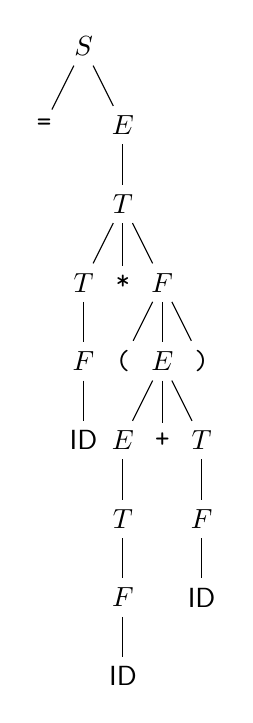
\begin{tikzpicture}
    \node (N0) at (0,0) {$\tteq$};
    \node (N1) at (0.5,1) {$S$};
    \node (N2) at (1,0) {$E$};
    \node (N3) at (1,-1) {$T$};
    \node (N4) at (0.5,-2) {$T$};
    \node (N5) at (1,-2) {$\ttmu$};
    \node (N6) at (1.5,-2) {$F$};
    \node (N7) at (1,-3) {$\texttt{(}$};
    \node (N8) at (1.5,-3) {$E$};
    \node (N9) at (2,-3) {$\texttt{)}$};
    \node (N10) at (0.5,-3) {$F$};
    \node (N11) at (0.5,-4) {$\textsf{ID}$};
    \node (N12) at (1,-4) {$E$};
    \node (N13) at (1.5,-4) {$\ttpl$};
    \node (N14) at (2,-4) {$T$};
    \node (N15) at (1,-5) {$T$};
    \node (N16) at (2,-5) {$F$};
    \node (N17) at (2,-6) {$\textsf{ID}$};
    \node (N18) at (1,-6) {$F$};
    \node (N19) at (1,-7) {$\textsf{ID}$};
    \path[-] (N1) edge (N0) (N1) edge (N2);
    \path[-] (N2) edge (N3) (N3) edge (N4) (N3) edge (N5) (N3) edge (N6);
    \path[-] (N4) edge (N10) (N10) edge (N11);
    \path[-] (N6) edge (N7) (N6) edge (N8) (N6) edge (N9);
    \path[-] (N8) edge (N12) (N8) edge (N13) (N8) edge (N14);
    \path[-] (N12) edge (N15) (N15) edge (N18) (N18) edge (N19);
    \path[-] (N14) edge (N16) (N16) edge (N17);
\end{tikzpicture}
\end{document}